\documentclass[titlepage,a4paper]{article}

\usepackage{a4wide}
\usepackage[colorlinks=true,linkcolor=black,urlcolor=blue,bookmarksopen=true]{hyperref}
\usepackage{bookmark}
\usepackage{fancyhdr}
\usepackage[spanish]{babel}
\usepackage[utf8]{inputenc}
\usepackage[T1]{fontenc}
\usepackage{graphicx}
\usepackage{float}
\usepackage{parskip}
\pagestyle{fancy} % Encabezado y pie de página
\fancyhf{}
\fancyhead[L]{TP1 -Grupo 6}
\fancyhead[R]{Análisis Numérico I - FIUBA}
\renewcommand{\headrulewidth}{0.4pt}
\fancyfoot[C]{\thepage}
\renewcommand{\footrulewidth}{0.4pt}

\newcommand{\HRule}{\rule{\linewidth}{0.5mm}}

\begin{document}
\begin{titlepage} % Carátula
	
\includegraphics[width=0.75\textwidth]{logofiuba.jpg}\\[4cm] 
    \centering
    \textsc{\LARGE Análisis Numérico I}\\[0.5cm]
    \textsc{\Large Primer cuatrimestre de 2021 }\\[0.5cm]  
    \HRule \\[0.4cm]
    {\huge \bfseries Trabajo Práctico 1: Búsqueda de raíces}\\[0.3cm]
    \HRule \\[2cm]
  	\Large
  	\begin{tabular}{ | l | l | l | }
  	    \hline
  	     Alumno & Número de padrón & Email \\ \hline
  	     BOCACCIO, Agustina & 106393 & abocaccio@fi.uba.ar \\
  	     SINGER, Joaquín & 105854 & josinger@fi.uba.ar \\
  	     LAZZARO, Melina & 105931 & mlazzaro@fi.uba.ar\\
  	     \hline
  	\end{tabular}
  	\vfill
            {\Large Curso: Sassano}\\
            {\Large Corrector: VERA GUZMAN, Ramiro}\\
            {\Large Lenguaje de programación utilizado: python}\\
  	\vfill
  	{\large 26 de Mayo de 2021}
\end{titlepage}

\tableofcontents % Índice general
\newpage
\section{Introducción}
El presente informe sera utilizado para especificar y analizar lo realizado en el Trabajo Practico 1 de Análisis Numérico I, en el cual se estudiaron métodos de búsqueda de raíces y su aplicación en diferentes problemas planteados.

\section{Objetivos}
Se estudian distintos métodos de búsqueda de raíces desarrollando los algoritmos de \textbf{Newton Raphson}, \textbf{serie de Leibniz}, \textbf{Newton Raphson modificado}, \textbf{Método de la Secante} y \textbf{Bisección}. Estos métodos fueron utilizados para hallar $\pi$, hallar raíces de tres funciones determinadas y para ayudar a un ser querido. Se realizará una comparativa entre los mismos analizando ventajas y desventajas de cada uno, también calculando su orden de convergencia y constante asintótica.

\section{Especificaciones sobre el desarrollo del trabajo}


\subsection{Método para seres queridos}
Se busca aplicar uno de los métodos vistos en clase en algo de la vida cotidiana para ayudar a un ser querido.
Se decidió utilizar el \textbf{método de la bisección} ya que es fue considerado como el mas sencillo de aplicar en lo cotidiano al ser el mas intuitivo y no necesitar hacer cálculos complejos de funciones y derivadas. Lo aplicamos para ayudar a un hermano/a pequeño a aprender a usar un diccionario y detallamos el proceso y las conclusiones en el archivo \verb|TP1_ramiro_6_2021_05_26.ipynb|. 

Este ejercicio permitió aplicar uno de los métodos aprendidos (en este caso el de la bisección), llevándolo a un plano mas cotidiano, reforzando el aspecto teórico aprendido durante las clases.



\subsection{Hallar \texorpdfstring{$\pi$}p por dos caminos}
El objetivo de esta parte es encontrar $\pi$ usando la \textbf{serie de Leibniz} y el método de búsqueda de raíces de \textbf{Newton-Raphson} en 64 y 32 bits, con la máxima precisión de la herramienta en el caso de Newton Raphson y con distinta cantidad de iteraciones en Leibniz.

Para Newton Raphson fue utilizada la función $\sin(x)$, que cumple con las condiciones del método ya que es continua al igual que su derivada, y la misma no se anula en $\pi$. La semilla elegida fue $x_0=3$ ya que el método además requiere una semilla que esté lo suficientemente cerca de la raíz.

\begin{figure}[H]
  \centering
    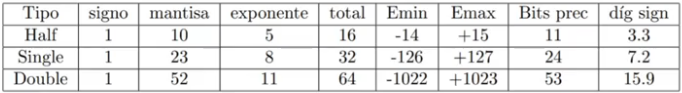
\includegraphics[width=0.75\textwidth]{tablita.png}
      \caption{Precisión de los tipos de dato en python}
\end{figure}
Se puede observar que en 64 bits python nos asegura 15 dígitos significativos, y en el caso de 32 bits, 7 dígitos significativos.

Además, fue utilizada una calculadora casio \verb|fx-570LA X| para obtener $\pi$ con ambos métodos y el error indicado en su manual.

Frente a los resultados obtenidos, se puede obtener como conclusión que, de entre los métodos utilizados para hallar $\pi$ en esta sección, el de Newton-Raphson en una arquitectura de 63 bits fue el mas óptimo, ya que se obtuvo una mejor aproximación, con un error menor y con menos iteraciones.

Todo lo mencionado, los resultados y la implementación de los métodos se encuentran detallados en el archivo entregado.


\subsection{Búsqueda de raíces}
En esta sección del trabajo se utilizaron los diferentes métodos aprendidos en clases para hallar las raíces de tres funciones y estudiar la convergencia de cada uno.
Estos son:
\begin{itemize}
    \item Método de Newton- Raphson
    \item Método de Newton-Raphson modificado
    \item Bisección
    \item Método de la secante
\end{itemize}
Para estudiar estos métodos y usarlos en la búsqueda de raíces, se comenzó por graficar las funciones en el intervalo que se pidió estudiar, y luego se desarrollaron los algoritmos de los métodos en Python.

Una vez desarrollados los algoritmos de los métodos, fueron usados para hallar la raíz de cada una de las funciones en el intervalo solicitado. Como criterio de paro se todos los métodos se usaron las cotas de error $1*10^{-5}$ y $1*10^{-13}$, es decir que el modulo de la diferencia entre dos iteraciones sucesivas sea menor a ese valor. Además, se uso $x_0=1,0$ como semilla para Newton-Raphson y Newton-Raphson modificado, y a los extremos del intervalo (0 y 2) como semillas del método de la secante.

En la función 3, se observó que con la o las semillas utilizadas en el método de Newton-Raphson, el de Newton-Raphson modificado, y el de la secante, estos procedimientos no pudieron converger. El motivo de esto fue explicado en el archivo entregado, junto con el nuevo calculo con este método con mejores semillas (elegidas basada en el gráfico de la función en este caso, pero también se podría obtener una semilla mejor usando el método de la bisección primero y a partir de allí usar Newton-Raphson).

En la ultima parte de este enunciado fueron implementados algoritmos para hallar el orden de convergencia y la constante asintótica para cada método con las diferentes funciones y las distintas cota de error. Ver las secciones \textbf{Gráficos del orden de convergencia con ambas cotas} y \textbf{Gráficos de la constante asintótica con ambas cotas}.

En esta parte del trabajo se pudieron observar las ventajas y desventajas del uso de cada método de búsqueda de raíces para diferentes funciones. El método de Newton-Raphson es muy poderoso por ser el de mayor convergencia (cuadrática para raíces simples), sin embargo para usarlo se necesita la derivada de la función estudiada, tiene convergencia lineal para raíces dobles y necesita de una buena aproximación inicial. Esto ultimo se debe a que de no tener una buena semilla, el método no va a converger, lo cual lo diferencia del de la bisección, el cual, a pesar de hacerlo mas lento, (linealmente), siempre converge. El otro procedimiento estudiado, el de la secante, tiene mayor convergencia que el de la bisección, pero menor que el de Newton-Raphson, y como este, necesita una buena aproximación inicial (y en su caso, no solo una, sino dos semillas) para converger. Sin embargo, tiene la ventaja de que no precisa la derivada de la función que se esta analizando. 

\newpage
\subsubsection{Gráficos del orden de convergencia con ambas cotas}
\begin{figure}[H]
  \centering
    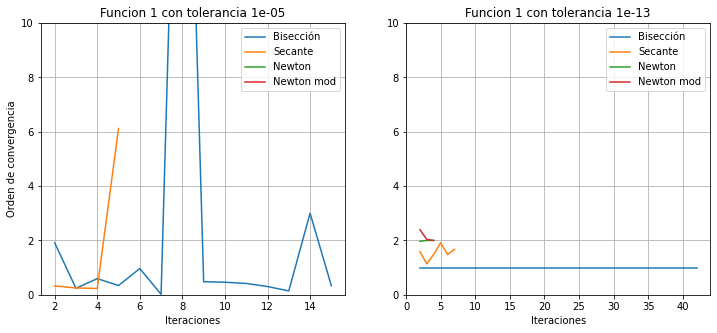
\includegraphics[width=0.9\textwidth]{converf1.png}
\end{figure}
\begin{figure}[H]
  \centering
    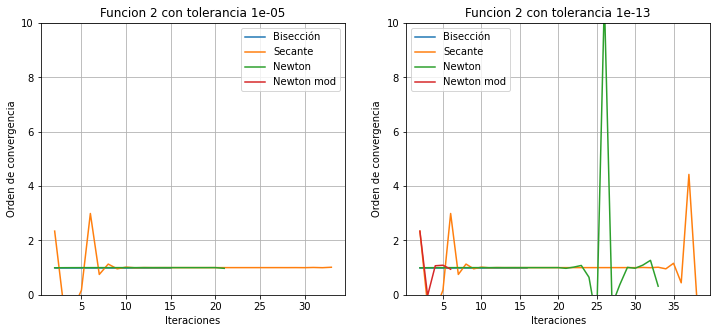
\includegraphics[width=0.9\textwidth]{converf2.png}
\end{figure}
\begin{figure}[H]
  \centering
    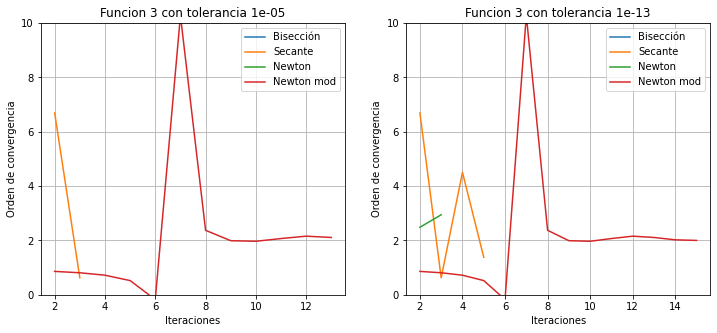
\includegraphics[width=0.9\textwidth]{converf3.png}
\end{figure}

\subsubsection{Gráficos de la constante asintótica con ambas cotas}
\begin{figure}[H]
  \centering
    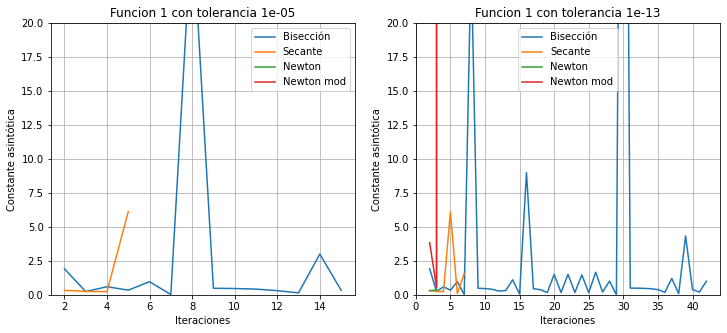
\includegraphics[width=0.9\textwidth]{asinf1.png}
\end{figure}
\begin{figure}[H]
  \centering
    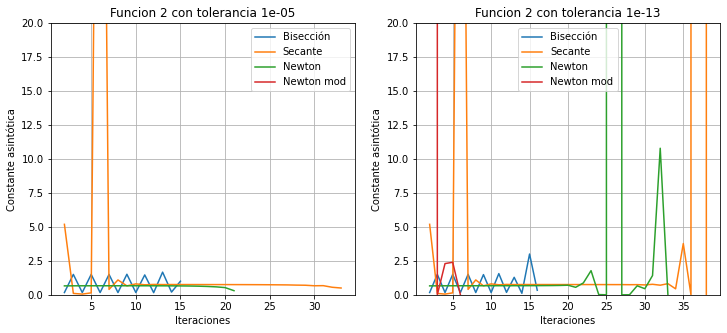
\includegraphics[width=0.9\textwidth]{asinf2.png}
\end{figure}
\begin{figure}[H]
  \centering
    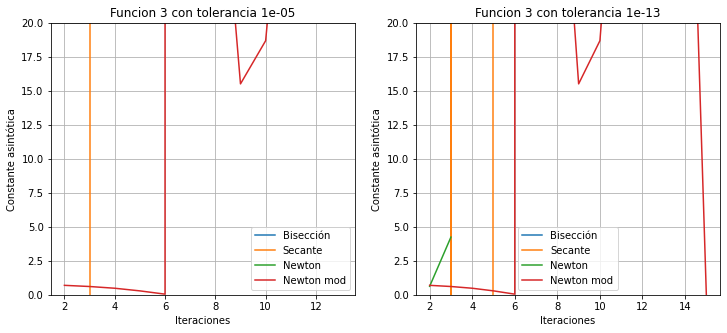
\includegraphics[width=0.9\textwidth]{asinf3.png}
\end{figure}

\newpage
Los casos donde no se ven graficados algunos métodos es porque convergen demasiado rápido y no hay suficiente información para hacer los cálculos.
No se pueden sacar conclusiones definitivas con respecto a la convergencia de cada método ya que teóricamente se calcula con infinitas iteraciones, cosa que es imposible para una computadora. Aumentar el número de iteraciones tampoco sería viable ya que llegará un momento en que la diferencia entre iteraciones será tan pequeña que harán underflow.


\section{Conclusiones}
Frente a las soluciones, aplicaciones y resultados obtenidos en el trabajo, se pueden determinar conclusiones basadas en los mismos. 

En la primera parte del trabajo se pudo encontrar una forma de aplicar uno de los métodos aprendidos a un problema de la vida cotidiana, lo cual permitió darle un uso practico y mas cercano a lo estudiado, mas allá del aspecto teórico del mismo. El uso de la bisección hizo que el ser querido solucione de forma mas eficiente su problema, ya que el niño/a hubiese tardado mas en leer hoja por hoja el diccionario que utilizando el método que se le fue dado. 

De la segunda parte del trabajo, en la cual se hallo $\pi$ mediante diferentes métodos, se puede concluir que el método de Newton-Raphson en una arquitectura de 64 bit fue el que obtuvo la mejor aproximación con un error mas pequeño que Newton-Raphson de 32 bit y Leibniz (en la calculadora o con la implementación de 64 bit), y también con una menor cantidad de iteraciones. Esto se debe a que la arquitectura de 64 bit proporciona una mayor precisión numérica, lo cual permite tener un error menor, pero nunca cero, ya que como fue explicado en el trabajo, el numero $\pi$ no es una constante para la computadora, porque cada número en ella se representa mediante un número finito de dígitos, y al ser $\pi$ irracional, su representación va a variar y va a tener un error determinado.

De la tercera parte se puede concluir que cada método de búsqueda de raíces tiene sus ventajas y desventajas, ya que si bien teóricamente Newton-Raphson tiene una convergencia mayor, tiene mas requisitos y en algunos casos, como sucede en este caso con la función 3, se tendrá que probar con distintas semillas para que pueda converger y no siempre se realizaran menos iteraciones que en los demás métodos. 
Las constantes asintóticas y orden de convergencia calculados mostraron no ser consistentes y dependen fuertemente de las condiciones iniciales como la función y semillas, además del número de iteraciones.

\newpage
\section{Referencias}
[1] Apuntes del curso Análisis numérico 1 - curso Sassano - Facultad de Ingeniería - Universidad de Buenos Aires - 2021.

[2] \verb|https://es.wikipedia.org/wiki/Serie_de_Leibniz|

\end{document}
